\documentclass[twoside,english, a4paper, 12pt]{uiofysmaster}
% \usepackage{biblatex}

\author{Anders Hafreager}
\title{\uppercase{Flow in nanoporous media}}
\date{October 2013}

\usepackage{listings}
\usepackage{xcolor}
\usepackage{amsmath}
\usepackage{amssymb}
% \usepackage[hidelinks]{hyperref}
\usepackage{hyperref}
\usepackage[T1]{fontenc}
\usepackage{bbold}
\usepackage{simplewick}
\usepackage[squaren]{SIunits}
\usepackage{sidecap}
\usepackage[titletoc]{appendix}

\definecolor{grey}{rgb}{0.98,0.98,0.98}
\definecolor{codeRed}{rgb}{0.5, 0.027, 0.02}

% Code parameters
\lstset{language=c++}
\lstset{basicstyle=\small}
\lstset{backgroundcolor=\color{white}}
\lstset{frame=single}
\lstset{stringstyle=\ttfamily}
\lstset{keywordstyle=\color{codeRed}\bfseries}
\lstset{commentstyle=\itshape\color{gray}}
\lstset{showspaces=false}
\lstset{showstringspaces=false}
\lstset{showtabs=false}
\lstset{breaklines}

\setlength{\parskip}{11pt}
\setlength{\parindent}{0mm}

\lstset{
language=Python,
basicstyle=\footnotesize
frame=single,
backgroundcolor=\color{grey}
}

\lstset{
language=Matlab,
basicstyle=\footnotesize,
frame=single,
backgroundcolor=\color{grey}
}

\lstset{
language=C++,
backgroundcolor=\color{grey}
}

\lstdefinelanguage{GLSL}
{
sensitive=true,
morekeywords=[1]{
attribute, const, uniform, varying,
layout, centroid, flat, smooth,
noperspective, break, continue, do,
for, while, switch, case, default, if,
else, in, out, inout, float, int, void,
bool, true, false, invariant, discard,
return, mat2, mat3, mat4, mat2x2, mat2x3,
mat2x4, mat3x2, mat3x3, mat3x4, mat4x2,
mat4x3, mat4x4, vec2, vec3, vec4, ivec2,
ivec3, ivec4, bvec2, bvec3, bvec4, uint,
uvec2, uvec3, uvec4, lowp, mediump, highp,
precision, sampler1D, sampler2D, sampler3D,
samplerCube, sampler1DShadow,
sampler2DShadow, samplerCubeShadow,
sampler1DArray, sampler2DArray,
sampler1DArrayShadow, sampler2DArrayShadow,
isampler1D, isampler2D, isampler3D,
isamplerCube, isampler1DArray,
isampler2DArray, usampler1D, usampler2D,
usampler3D, usamplerCube, usampler1DArray,
usampler2DArray, sampler2DRect,
sampler2DRectShadow, isampler2DRect,
usampler2DRect, samplerBuffer,
isamplerBuffer, usamplerBuffer, sampler2DMS,
isampler2DMS, usampler2DMS,
sampler2DMSArray, isampler2DMSArray,
usampler2DMSArray, struct},
morekeywords=[2]{
radians,degrees,sin,cos,tan,asin,acos,atan,
atan,sinh,cosh,tanh,asinh,acosh,atanh,pow,
exp,log,exp2,log2,sqrt,inversesqrt,abs,sign,
floor,trunc,round,roundEven,ceil,fract,mod,modf,
min,max,clamp,mix,step,smoothstep,isnan,isinf,
floatBitsToInt,floatBitsToUint,intBitsToFloat,
uintBitsToFloat,length,distance,dot,cross,
normalize,faceforward,reflect,refract,
matrixCompMult,outerProduct,transpose,
determinant,inverse,lessThan,lessThanEqual,
greaterThan,greaterThanEqual,equal,notEqual,
any,all,not,textureSize,texture,textureProj,
textureLod,textureOffset,texelFetch,
texelFetchOffset,textureProjOffset,
textureLodOffset,textureProjLod,
textureProjLodOffset,textureGrad,
textureGradOffset,textureProjGrad,
textureProjGradOffset,texture1D,texture1DProj,
texture1DProjLod,texture2D,texture2DProj,
texture2DLod,texture2DProjLod,texture3D,
texture3DProj,texture3DLod,texture3DProjLod,
textureCube,textureCubeLod,shadow1D,shadow2D,
shadow1DProj,shadow2DProj,shadow1DLod,
shadow2DLod,shadow1DProjLod,shadow2DProjLod,
dFdx,dFdy,fwidth,noise1,noise2,noise3,noise4,
EmitVertex,EndPrimitive},
morekeywords=[3]{
gl_VertexID,gl_InstanceID,gl_Position,
gl_PointSize,gl_ClipDistance,gl_PerVertex,
gl_Layer,gl_ClipVertex,gl_FragCoord,
gl_FrontFacing,gl_ClipDistance,gl_FragColor,
gl_FragData,gl_MaxDrawBuffers,gl_FragDepth,
gl_PointCoord,gl_PrimitiveID,
gl_MaxVertexAttribs,gl_MaxVertexUniformComponents,
gl_MaxVaryingFloats,gl_MaxVaryingComponents,
gl_MaxVertexOutputComponents,
gl_MaxGeometryInputComponents,
gl_MaxGeometryOutputComponents,
gl_MaxFragmentInputComponents,
gl_MaxVertexTextureImageUnits,
gl_MaxCombinedTextureImageUnits,
gl_MaxTextureImageUnits,
gl_MaxFragmentUniformComponents,
gl_MaxDrawBuffers,gl_MaxClipDistances,
gl_MaxGeometryTextureImageUnits,
gl_MaxGeometryOutputVertices,
gl_MaxGeometryOutputVertices,
gl_MaxGeometryTotalOutputComponents,
gl_MaxGeometryUniformComponents,
gl_MaxGeometryVaryingComponents,gl_DepthRange},
morecomment=[l]{//},
morecomment=[s]{/*}{*/},
morecomment=[l][keywordstyle4]{\#},
}

% ------------------------------------------------- COLOR BOX
                                                                

\renewcommand{\vec}{\mathbf}
\newcommand{\mat}{\mathbf}
\newcommand{\F}{\mathbf{F}}
\newcommand{\E}{\mathbf{E}}
\newcommand{\B}{\mathbf{B}}
\newcommand{\J}{\mathbf{J}}
\newcommand{\R}{\mathbf{R}}
\newcommand{\avec}{\mathbf{a}}
\newcommand{\rvec}{\mathbf{r}}
\newcommand{\vvec}{\mathbf{v}}
\newcommand{\xvec}{\mathbf{x}}
\newcommand{\diverg}{\nabla \cdot}
\newcommand{\curl}{\nabla \times}
\newcommand{\laplace}{\nabla^2}
\newcommand{\definition}{\emph}
\newcommand{\dpart}[2]{\frac{\partial #1}{\partial #2}}
\newcommand{\dd}[2]{\frac{\mathrm{d}#1}{\mathrm{d}#2}}
\newcommand{\unit}[1]{\hat {\vec{#1}}}

% Quantum stuff
\newcommand{\infint}{\int_{-\infty}^{\infty}}

% Equations
\newcommand{\bea}{\begin{eqnarray*}}
\newcommand{\eea}{\end{eqnarray*}}
\newcommand{\beq}{\begin{equation}}
\newcommand{\eeq}{\end{equation}}


% \usepackage{autocite}
\usepackage[]{biblatex}
\bibliography{Bibliography/bibliography.bib}

\begin{document}

\maketitle
\clearpage

\begin{abstract}
This is an abstract text.
\end{abstract}
\begin{dedication}
  To someone
  \\\vspace{12pt}
  This is a dedication to my cat.
\end{dedication}
\begin{acknowledgements}
  I acknowledge my acknowledgements.
\end{acknowledgements}

\tableofcontents
\clearpage
\listoffigures
\clearpage
\listoftables

\begin{part}{Introduction}
\begin{chapter}{Introduction}
  \section{Introduction}


\subsection{Motivation}


\subsection{The structure of this thesis}


\section{My contribution}

\end{chapter}

\begin{chapter}{Background}
  \section{History of fluid mechanics and gas dynamics}
The history of any physical field is interesting in several ways. Physical questions usually start with one or more observations, the \textit{what}, and then the urge to understand \textit{why}. In science, \textit{why} is of course the question we ideally want to answer, but in many cases that is not achievable at first. An example is the statement of Kepler's three laws of planetary motion. Kepler had observations that he confirmed were indeed correct, but he did not know \textit{why} the planets behave like they do. Some 50 years later, Newton explained Kepler's three laws by his universal law og gravitation. This is the beauty of science, the \textit{why} is not required, just desired.\\
Another interesting part of the history is the amount of available information at the time of discoveries, which strongly affects their ability to develop new theories. Newton needed to create a theory that were in agreement with Kepler's laws, and Kepler needed his laws to agree with the observations that were done.\\
In this section, we will briefly discuss how the discoveries in fluid mechanics were done, and the questions that lead up to our current knowledge of the field. 

\subsection{The beginning in Greece}
The first scientific describtions of fluid mechanics dates back to Aristotle (384-322 B.C.) when he identified the continuum and dynamic drag in fluids.\cite{book:fluid_history} He wrote
\begin{quotation}
The continuous may be defined as that which is divisible into parts which are themselves divisible to infinity, as a body which is divisible in all ways. Magnitude divisible in one direction is a line, in three directions a body. And magnitudes which are divisible in this fashion are continuous. 
\end{quotation}
The idea of continuum is fundamental in most fluid mechanics theories and is a rather abstract concept that makes the mathematics work out beautifully. At the time of Aristotle, the mathematical framework was not yet established, so it was an impressive contribution to the field. The more intuitive drag force was described as
\begin{quotation}
It is impossible to say why a body that has been set in motion in a vacuum should ever come to rest. Why, indeed, should it come to rest at one place rather than another. As a consequence, it will either necessarily stay at rest, or if in motion, will move indefinitely unless some obstacle comes into collision with it.
\end{quotation}
For fluids in movement, the obstacle is the thing creating the drag force preventing the fluid to move freely. About a hundred years later, Archimedes (287-212 B.C.) published \textit{On Floating Bodies} where he discussed what is now known as \textit{Archimedes' principle} that states
\begin{quotation}
Any object, wholly or partially immersed in a fluid, is buoyed up by a force equal to the weight of the fluid displaced by the object.
\end{quotation}
Even today, more than 2000 years later, every high school student taking a physics course learn about Archimedes' principle. It is a simple and intuitive, yet remarkably powerful, statement that can easily be derived using Newtonian mechanics. 

\subsection{Conservation laws and the Navier-Stokes equations}
One can derive the Navier-Stokes equations (NSE) by assuming conservation of energy, mass and momentum ending up with\cite{batchelor2000introduction}
\begin{align}
	\rho \dpart {\vec v}{t} + \vec v\nabla\vec v = -\nabla p + \mu\nabla^2\vec v + \vec f,
\end{align}
where $\vec v$ is the fluid velocity, $\mu$ the viscosity and $\vec f$ is an external force (i.e. gravity). It is a set of coupled non-linear differential equations that can be seen as one vector differential equation. It has quite a few interesting analytically solvable solutions, but for most real systems, the geometry confining the fluid is so complex that it is solved on computers. A much used technique is to use a Finite Element Method (FEM) which works for arbitrary geometries. 

\subsection{The breakdown of contiinum}
A fundamental assumption in the NSE is that the space is continuous so that every point in space has well defined physical properties like density, velocity, temperature and pressure. This is known as the \textit{continuum hypothesis} and is invalid when the \textit{mean free path} $\lambda$, the average distance a particle moves between collisions, becomes large compared to some characteristic length $L$ in the system, i.e. the diameter of a channel. This property is quantified through the \textit{Knudsen number} which is defined as
\begin{align}
	Kn = \frac{\lambda}{L}.
\end{align}
For small Knudsen numbers (of order $10^{-2}$ or less), the contiinum hypthosis is valid and we can apply the Navier-Stokes equations\cite{karniadakis2005microflows}.
\subsection{Atomic models}
When the continuum hypothesis is invalid, we need another model describing the behaviour of the particles in our system. The first thing that might pop your mind might be to study the system at the atomic level. The physical set of rules that are controlling the atoms is of course quantum mechanics. The equations of motion and hence the dynamics of an atomic can in principle be calculated directly from quantum mechanics by solving Schrödinger's equation with perturbation theory, but the size of the system needs to be very small. An alternative, popular approach is to use a parameterized potential $U(\vec r^N)$, which is a function of the positions of all the atoms, and calculate the forces through the gradient of $U$. Newton's equations of motion is then integrated and the dynamics of the system are determined in a classical, deterministic way where important effects from quantum mechanics can be embedded in the potential. This method is called \textit{Molecular Dynamics} and is studied in chapter \ref{chap:md}. This method is computationally very expensive because it needs a detailed describtion of every atom in the system. For many problems, the specific details of each atom is not very important, but we want the statistical properties of the system.
\subsection{Statistical mechanics and the kinetic theory of gases}
We know from statistical mechanics that what dominates the macroscopic effects is the statistical behaviour of the system. One can derive the ideal gas law from pure statistical and combinatorial arguments with conservation of energy being the only physical concept\cite{ravndal2008statmech}. The idea is that it is the average properties of a system that are being observed wheras the actual state (i.e. all the positions and velocities of all atoms) of the system is not known. A physical system is often described as a distribution function $f(\vec r, \vec v; t)$ yielding the probability of finding an atom, or in general a particle in the volume element $d\vec r d\vec v$ at the time $t$. The dynamics of this function is described by the Boltzmann equation which is derived in section \ref{sec:boltzmann_equation}. From the Boltzmann equation, we can derive  the results we need to describe the properties of gases which will be input parameters to a model called Direct Simulation Monte Carlo (DSMC) which is studied in chapter \ref{chap:dsmc}. These results are called the kinetic theory of gases.
\subsection{Porous media}
A porous medium is a material with pores and channels (the pore network) available for fluids. Typical examples are sandstone and sponges, see figure \ref{fig:history_porous_media}. 
\begin{figure}[h]
\begin{center}
%\includegraphics[width=\textwidth, trim=0cm 0cm 0cm 0cm, clip]{figures/porous_media.png}
\label{fig:history_porous_media}
\end{center}
\caption{Porous media.}
\end{figure}

\subsection{Nanoporous media}

  \section{Applications}
\subsection{Shale gas extraction}
\subsection{Electronic devices}
  \section{Multi scale physics}

\subsection{Our world}
Throughout the history, from the ancient greeks up until today, humans have tried to understand the rules of our universe and how they affect what we see and experience every day. Today, we believe that everything is controlled by the rules of quantum mechanics, where some of its effects are visible even for the naked eye. An example is seen every summer during hot days while driving a car on a straight road, namely mirage. The warm road reflects light as if it's covered in water, so you can see the sky and oncoming cars on the road. This phenomena is fully explained by quantum electrodynamics and the fact that there is a temperature gradient in the air pointing from the asphalt and upwards. Light moves slower through dense air, and the air is less dense at high temperatures, so the light wants to travel closer to the asphalt. This means that the actual path the light takes is not a straight line, but is bent, see figure \ref{TODO}. The light is taking a shortcut. Mirage can be explained, or should I say modelled, by simpler ideas, but the actual reason arises from quantum mechanics. 

\subsection{Simulation of the universe}
Say we want to use our computers and simulate a universe very similar to our own. We will use all our knowledge about physics, so the fundamental theory we plug in is quantum mechanics. We need to account for relativistic effects, so we have to unify quantum theory with general theory of relativity first. A universe, even a tiny one, contains a lot of information, so the amount of required computer memory is enormous, but this is not our biggest problem. Time is usually discretized, so in order to solve the fundamental equations of unified relativistic quantum mechanics with today's techniques, we will probably need a very small timestep. Larger time scales, like the ones needed to compute cosmological properties of the universe, are therefore out of reach even with decades of Moore's law. 

\subsection{An ideal world}

\subsection{The weakest link}


\end{chapter}
\end{part}

\begin{part}{Molecular Dynamics}
  \begin{chapter}{Introduction}
  Molecular Dynamics is another numerical model that describes the behaviour of liquids, gases and solids at the finest scale of any classical model. We can study the dynamics of single atoms and how they interact with each other forming molecules and larger objects like advanced pore networks. The idea is simple and has been used since the time of Sir Isaac Newton in the 17th century when he formulated his laws of motion. With the knowledge of the relevant forces between the atoms, we can solve Newton's equations and calculate their dynamics.

We open this chapter by a short introduction to the model in section \ref{sec:md_model} before we explain how forces are calculated with the Lennard-Jones potential in section \ref{sec:md_forces}. With computed forces, we can integrate the atoms with Newton's laws following an time integration scheme which we discuss in section \ref{sec:md_time_integration}. The last section is concerned with how we measure physical quantities which will be very similar to what we did with DSMC in section \ref{sec:dsmc_measuring_physical_quantities}.
  \end{chapter}
  \section{c++-code}
  \section{F77-code}
\end{part}

\begin{part}{Direct Simulation Monte Carlo}

\begin{chapter}{Kinetic theory}
  \section{Origin}
  \section{The Boltzmann equation}
\label{sec:boltzmann_equation}
In the section \ref{sec:kinetic_theory_distribution_function}, we introduced the distribution function $f$ that describes the density in a $6N$ dimensional phase space. Now, if we know the distribution function at $t=0$, we could in principle compute any property of the system. But at a later time $t=\tau$, the distribution function might have changed, unless, of course, $\partial_t f = 0$ (in which the system would be in what we call an equilibrium state). We can, by applying conservation of probability, derive an equation of motion for $f$. This equation is called the Boltzmann equation. It describes how $f$ evolves through time by assuming that any change of density (read probability) around a point $(\vec r, \vec v)$ at the time $t$ must be due to
\begin{itemize}
	\item flow through a surface in the phase space,
	\item an external force, or
	\item internal collisions.
\end{itemize}
All three will change $f$ in different ways. For simplicity, we will first assume that the particles do not collide and derive the \textit{collisionless Boltzmann equation}. But do not worry, we will add the collision term later and end up with the full Boltzmann equation.

\subsection{The collisionless Boltzmann equation}
Consider the density around the phase space point $(\vec r,\vec v)$ at the time $t$. If we assume no forces, and that the total number of particles has not changed, a time $dt$ later, the density has moved to $(\vec r + \vec vdt, \vec v)$. Conservation of probability states that any change of $f$ within a volume $\Omega$ must flow through the boundary $\partial \Omega$
\begin{align}
	\frac{\dm }{\dm t}\int_\Omega f \dm \vec r \dm \vec v &= -\int_{\Omega_v}\dm \vec v\int_{\partial \Omega_r} f(\vec v\cdot \vec n_r) \dm S_r\\
	&= -\int_{\Omega_v}\dm \vec v\int_{\Omega_r} \nabla_\vec r\cdot(f\vec v) \dm \vec r = -\int_{\Omega} \nabla_\vec r\cdot(f\vec v) \dm \vec v\dm \vec r
\end{align}
which becomes
\begin{align}
	\dpart{f}{t} + \nabla_\vec r \cdot(f\vec v) = \dpart{f}{t} + \vec v\cdot\nabla_\vec r f = 0
\end{align}
since $\vec v$ is independent of $\vec r$. We can extend this equation by adding the effects of an external force $\vec F$ that changes the velocity in the same way as the position was changed above (except for the factor $1/m$)
\begin{align}
	\label{eq:collisionless_boltzmann}
	\dpart{f}{t} + \vec v\cdot\nabla_\vec r f + \nabla_\vec v \cdot \frac{\vec F}{ m}f = 0,
\end{align}
which we call the collisionless Boltzmann equation. It is a good approximation to describe the dynamics of very dilute gases where intermolecular collisions occur rarely. But we should not ignore collisions between particles, so as promised, we will now see that by treating collisions will appear as an additional term.
\subsection{The collision operator}
We consider a dilute gas so we can assume that only binary collisions occur (we ignore the contribution from collisions between three or more particles at a time). We also assume that the total energy and momentum is conserved in all collisions. Then consider two particles $i$ and $j$ moving towards each other with velocities $\vec v$ and $\vec v_1$, and relative velocity $\vec g = \vec v - \vec v_1$. We define particle $i$ as the \textit{incident} particle and $j$ as the \textit{target} particle. After the collision, the particles will have velocities $\vec v'$ and $\vec v_1'$ with relative velocity $\vec g' = \vec v' - \vec v_1'$. In order to make the calculations simpler, we change the frame of reference. If we choose the target particle as initial frame of reference, we see that the velocity of the incident particle becomes $\tilde {\vec v} = \vec g$ and $\tilde {\vec v}' = \vec g'$. Since momentum is conserved, we know that the relative velocity must remain constant $|\vec g| = |\vec g'|$ during the collision. The direction of $\vec g'$ is given by the angles $\phi$ and $\theta$ with $\hat {\vec z}$ along $\vec g$ and $\phi \in [0, 2\pi], \theta \in [0, \pi]$. We can express $\vec g'$ as
\begin{align}
	\vec g' = \vec g - 2\unitvector e(\unitvector e\cdot\vec g),
\end{align}
where $\unitvector e$ is an arbitrary unit vector. \todo{Illustrate this with a figure?} If we multiply by $\unitvector e$, we see that 
\begin{align}
	\unitvector e\cdot \vec g' = \unitvector e\cdot\left[\vec g - 2\unitvector{e}(\unitvector e\cdot\vec g)\right] = -\unitvector e \cdot \vec g
\end{align}
which gives the symmetric relation
\begin{align}
	\vec g = \vec g' - 2\unitvector e(\unitvector e\cdot\vec g').
\end{align}
The angle between $\vec g$ and $\vec g'$ is $\theta$, so
\begin{align}
	\vec g'\cdot \vec g = g^2\cos\theta = g^2(1 - 2\cos \chi),
\end{align}
where $\chi$ is the angle between $\unitvector e$ and $\vec g$ which gives the relation
\begin{align}
	\theta = \pi - 2\chi.
\end{align}
We now define the solid angle element $\dm\Omega=\sin\theta \dm\theta \dm\phi$ about $\vec g'$ 
\begin{align}
	g \dm\Omega &= g\sin\theta \dm\theta \dm\phi = 2g\sin(\pi - 2\chi)\dm\chi \dm\phi\\
	&= 4g\cos\chi\sin\chi \dm\chi \dm\phi = 4\left|\unitvector e\cdot\vec g\right|\sin\chi \dm\chi \dm\phi\\
	&= 4\left|\unitvector e\cdot\vec g\right|\dm^2e,
\end{align}
where $\dm^2e = \sin\chi \dm\chi \dm\phi$ is a solid angle element about $\unitvector e$. In the following, we will calculate the scattering cross section which is the \textit{area} that describes the likelyhood of an incident particle being scattered by the target particle. We denote the number density $\rho_n$ and find that the incident flux is $\rho_n g$. The rate $h_{\dm\Omega}'$ of scattered particles into $\dm\Omega$ is
\begin{align}
	\label{eq:partial_scattering_rate}
	h_{\dm\Omega}' = \rho_n g\sigma \dm\Omega,
\end{align}
where the proportionality constant $\sigma$ is the cross section. We might have several target particles colliding independently of each other which will contribute to the scattering rate. If we have $n_t$ such particles, we obtain the total scattering rate $h_{\dm\Omega}$ by multiplying \eqref{eq:partial_scattering_rate} by $n_t$
\begin{align}
	h_{\dm\Omega} = n_t\rho_n g\sigma \dm\Omega.
\end{align}
The \textit{differential} cross section $\sigma$ depends on $\vec g$ and $\vec g'$, so we denote it as $\sigma = \sigma(\vec g\rightarrow \vec g')$, whereas the \textit{total} cross section $\sigma_T$ is given by integrating over all solid angles
\begin{align}
	\sigma_T = \int \sigma \dm\Omega.
\end{align}
We will now look at particles with velocities in the range $[\vec v, \vec v + \dm\vec v]$ incident on target particles with velocities in the range $[\vec v_1, \vec v_1 + \dm\vec v_1]$. The incident flux is $gf(\vec v,\vec r)\dm\vec v$ and the number of target particles is $f(v_1,\vec r)\dm\vec v_1\dm\vec r$. The rate at which particles with velocity $\vec v_1$ are scattered by particles with velocity $\vec v$ is \todo{Check if these $f$'s should be normalized}
\begin{align}
	f(\vec v)f(\vec v_1) g \sigma \dm\Omega \dm\vec v \dm\vec v_1 \dm\vec r = f(\vec v)f(\vec v_1)4\left|\unitvector e\cdot \vec g\right| \sigma \dm^2e \dm \vec v \dm\vec v_1 \dm \vec r.
\end{align}
The rate of loss is the rate of which particles in $\dm\vec v\dm\vec r$ are being hit by other particles. We can calulate this by integrating over all solid angles $\dm^2 e$ and incident velocities $\dm \vec v$
\begin{align}
	\text{rate of loss} = \left[\int f(\vec v)f(\vec v_1)4\left|\unitvector e \cdot \vec g \right|\sigma \dm^2 e\dm \vec v_1\right]\dm \vec v\dm \vec x.
\end{align}
We also have the inverse event, incident particles with velocity $\vec v'$ hitting target particles with velocity $\vec v_1'$ so that the final velocity of the target particles is $\vec v$. This is calculated with the same idea
\begin{align}
	\text{rate of gain} = \left[\int f(\vec v')f(\vec v_1')4\left|\unitvector e \cdot \vec g \right|\sigma \dm^2 e\dm \vec v_1\right]\dm\vec v\dm\vec x,
\end{align}
since $|\unitvector e\cdot \vec g| = |\unitvector e\cdot \vec g'|$ and $\dm\vec v'\dm\vec v_1' = \dm\vec v\dm\vec v_1$. The total change in the distribution function is given by the functional $J[f]$
\begin{align}
	J[f] &= \int \dm\vec v_1 \dm^2 e4|\unitvector e\cdot\vec g|\sigma[f'f_1' - ff_1]\\
	&= \int \dm\vec v_1 \dm\Omega g \sigma[f'f_1' - ff_1],
\end{align}
where $f = f(\vec r, \vec v, t)$ and $f_1 = f(\vec r, \vec v_1, t)$. The full Boltzmann equation is then given by
\begin{align}
	\label{eq:boltzmann_equation}
	\dpart{f}{t} + \vec v\cdot \nabla_\vec r f + \frac{\vec F}{m}\cdot\nabla_\vec v f = J[f].
\end{align}
In the derivation of the collision operator $J[f]$, we assumed binary collisions only. This is a decent approximation that holds for low densities. By defining the force range $D$ and the dimensionless parameter $\nu = \rho_n D^3$, the Boltzmann equation is valid when $\nu$ is small \cite{mclennan1989introduction}. $D^3$ defines a volume around a particle in which the forces cannot be neglected. This makes $\nu$ the average number of particles within that volume. If that number is small (less than unity) then we can safely neglect collisions between three or more particles.
\section{\textit{H}-theorem}

Boltzmann's $H$-theorem is a powerful result that gives us all the theoretical tools we need to implement the DSMC method. We define the $H$-function as
\begin{align}
	H(t) = \langle \ln f \rangle = \int f(\vec r, \vec v, t)\ln f(\vec r, \vec v, t)d\vec r d\vec v
\end{align}
and differenciate with respect to time
\begin{align}
	\frac{dH}{dt} = \int \dpart{f}{t}\ln f d\vec r d\vec v + \int \dpart{f}{t} d\vec r d\vec v = \int \dpart{f}{t}\ln f d\vec r d\vec v
\end{align}
where we have used that the number of particles is conserved
\begin{align}
	\int \dpart{f}{t}d\vec r d\vec v = \frac{d}{dt} \int fd\vec r d\vec v = \frac{dN}{dt} = 0.
\end{align}
We multiply the Boltzmann equation by $\ln f$ and integrate
\begin{align}
	% \int \dpart{f}{t}\ln f d\vec r d\vec v = -\int (\ln f)\vec v\cdot \nabla_\vec r f d\vec r d\vec v - \int (\ln f) {\vec F\over m}\cdot \nable_\vec v f d\vec rd\vec v + \int \ln f J[f] d\vec r d\vec v
	balle
\end{align}

\section{Maxwell-Boltzmann distribution as equilibrium}
\label{sec:maxwell_boltzmann_distribution}
\begin{align}
	\label{eq:maxwell_boltzmann_distribution}
	P(v_i)\dm {v_i} = \sqrt\frac{m}{ 2\pi k_BT}e^\frac{-mv_i^2}{ 2k_BT}\dm {v_i},
\end{align}
\section{Mean free path}
\label{sec:mean_free_path_calculation}
The collision frequency can be calculated through the mean free path, which is the average distance a molecule travels between collisions. The mean free path for a gas is estimated by looking at the \textit{effective collision area}, see figure \ref{fig:effective_collision_area}. The effective collision area is then
\begin{align}
	A = \pi d^2,
\end{align}
where $d$ is the molecular diameter. Two molecules with velocities $\vec v_1$ and $\vec v_2$ have the relative velocity $\vec v_{rel} = \vec v_1 - \vec v_2$. The norm is given by
\begin{align}
	v_{rel} &= \sqrt{\vec v_{rel}\cdot \vec v_{rel} } = \sqrt{ (\vec v_1 - \vec v_2)(\vec v_1 - \vec v_2)}\\
	&= \sqrt{\vec v_1\cdot \vec v_1 - 2\vec v_1\vec v_2 + \vec v_2\vec v_2}.
\end{align}
The average relative velocity is calculated by assuming that the velocities are completely random and hence not correlated, and that the molecules have the same mean speed $\langle v\rangle$
\begin{align}
	\bar v_{rel} &= \sqrt{\vec v_1^2 + \vec v_2^2} = \sqrt 2 \langle v\rangle,
\end{align}li
During a time $\tau$ and average relative molecular velocity $\sqrt 2 \langle v\rangle$, the total volume sweeped out by the particle is given as
\begin{align}
	V = \sqrt 2 \pi d^2\langle v\rangle \tau,
\end{align}
which in turn gives the number of collisions during such a volume
\begin{align}
	\label{eq:num_collisions}
	n_{coll} = V\rho_n = \sqrt 2 \pi d^2\langle v\rangle \rho_n \tau,
\end{align}
where $\rho_n$ is the number density. The mean free path is then calculated as the length of the path divided by the number of collisions
\begin{align}
	\label{eq:mean_free_path}
	\lambda = \frac{\langle v\rangle \tau}{ \sqrt 2 \pi d^2\langle v\rangle \rho_n\tau} = \frac{1 }{ \sqrt 2 \pi d^2 \rho_n}
\end{align}
\section{Mean collision time}
\begin{align}
	\label{eq:coll_frequency}
	f_{coll} = \rho_n \pi \sigma^2 \langle v_r \rangle
\end{align}
  \section{The Chapman-Enskog method}

\end{chapter}

\begin{chapter}{Direct Simulation Monte Carlo}
  We now have the theoretical foundation we need to develop the first numerical model we will use to study flow in nanoporous media. It is called Direct Simulation Monte Carlo (DSMC), and is a stochastic particle model that has showed incredible predictive power for flow in the high Knudsen number regime. The model was developed by G. A. Bird in 1976 and was quickly picked up by engineers working in the field of aerospace. In the upper atmosphere (\unit{100}{\kilo\meter}), the mean free path of air is several meters. For space shuttles, this gives a Knudsen number of order unity since the size of its nose is of order meter \cite{alexander1997direct}. In the later years, the method has been widely used to study microflows which is our main concern in this thesis. In 1992, the model was proved to converge towards a solution of the Boltzmann equation (equation \eqref{eq:boltzmann_equation}) in the limit where the timestep $\Delta t\rightarrow 0$ and the number of particles $M\rightarrow \infty$.\\
We start the chapter by introducing the model and its basic philosophy. The model has two two crucial parts, collisions between particles which is discussed in section \ref{sec:dsmc_collisions_model}, and how the particles interact with the surface. The latter is covered in section \ref{sec:surface_interactions}. Another important subject is of course how we measure physical quantities like temperature and energy. This is described in section \ref{sec:dsmc_measuring_physical_quantities}. In section \ref{sec:dsmc_pressure} we have a longer discussion about the pressure and argue that a DSMC gas actually satisfies the ideal gas equation of state. We also derive a relationship between a given pressure difference $\Delta P$ and a constant force allowing us to induce flow in the system without needing large gradients in the density or temperature. We then have a brief comment about the numerical stability and how the timestep and collision cell size introduce errors in transport coefficients. We complete the chapter by discussing how we determine whether or not a system has reached a steady state in section \ref{sec:dsmc_steady_state}. The implementation of all these steps are explained in detail in chapter \ref{chap:dsmc_implementation}.
  \section{Surface interactions}
\label{sec:surface_interactions}
The effects of surface interactions become significant as the pore sizes decrease. For very small pores, the number of atoms near the surface is comparable with total number of atoms. In MD, these effects are already taken care of through the atomic forces, but in DSMC, we need a surface interaction model. We discuss three different models in this section. The main property of these models is to perform a statistically correct energy and momentum transfer between the wall and the colliding particles. In DSMC, we are only interested in the macroscopic details of these collisions. There are two important parameters that incorporates the differences between different gases and surfaces; the normal and tangential accomodation coefficients.
\subsection{Accomodation coefficients}
When a particle hits a wall with energy $E_i$, some of the energy might be transferred to the wall resulting in an energy change $\Delta E$. On average, we can define the \textit{normal accomodation coefficient} 
\begin{align}
	\sigma_n = \frac{E_i - E_r}{E_i - E_w},
\end{align}
where $E_i$ is the energy of the incoming particles, $E_r$ is the energy of the outging molecules and $E_w$ is the energy corresponding to the surface temperature $T_w$. A thermal accomodation coefficient equal to zero would mean that there is no energy exchange, and we will get the specular wall model described below. $\sigma_T=1$ on the other hand means that all the reflected particles have energies corresponding to the surface temperature. This is what we call the thermal wall (or diffuse reflection\cite{karniadakis2005microflows}), and there is no correlation between the incoming and outgoing velocities. More intricate models make use of other values of the accomodation coefficients so the particles \textit{remember} their incoming velocities.\\
We can also define the \textit{tangential momentum accomodation coefficient}
\begin{align}
	\sigma_t = {\tau_i - \tau_r\over \tau_i - \tau_w},
\end{align}
where $\tau_i$ and $\tau_r$ are the incoming and outgoing tangential momentum and $\tau_w$ is the momentum of the wall. For stationary surfaces we have $\tau_w=0$.

\subsection{Specular wall}
The specular wall behaves just like a classical mirror. The colliding objects are reflected so that the normal component of the velocity is reversed while the tangential components remain unchanged. There is no exchange of energy with the wall. 

\subsection{Thermal wall}
If we instead think of the wall as an object with a given temperature $T_w$, we can imagine that the particles go into the wall, collide with the wall atoms as a random walk, and return with no correlation with the incoming velocity. We can then choose a new, random velocity vector from a distribution so that the gas temperature converges to the wall temperature. This distribution has to reflect the fact that faster particles collide more often with the surface. A distribution that satisfies this property is the biased Maxwell-Boltzmann distribution given as
\begin{align}
	P_n(v_n) = {m\over kT_w}v_n e^{-mv_n^2/2kT_w}
\end{align}
for the velocity component normal on the surface and
\begin{align}
	P_t(v_t) = \sqrt{m\over 2\pi kT_w}e^{-mv_t^2/2kT_w},
\end{align}
for the tangential component. Here $m$ is the mass of the particle and $k$ is Boltzmann's constant\cite{alexander1997direct}. This distribution does not obey detailed balance since the incoming velocity is completely uncorrelated to the outgoing velocity. It is computationally inexpensive and is much used in the literature. 
\subsection{The Cercignani-Lampis model}
Another more realistic model is the Cercignani-Lampis model which was derived requiring detailed balance and wall isotropy\cite{cowling1974cercignani}. The probability of going from an incoming velocity $\vec v'$ to an outgoing velocity $\vec v$ is given as
\begin{align}
	\nonumber
	P(\vec v'\rightarrow \vec v) &= \frac{2\sigma_n\sigma_t(2-\sigma_t)\beta_w^4}{\pi}\\
	\nonumber
	&\times\exp\Big(-\beta_w^2\frac{v_n^2 + (1-\sigma_n)(v_n')^2}{\sigma_n} - \beta_w^2\frac{(v_t - (1 - \sigma_t)v_t')^2}{\sigma_t(2 - \sigma_t)}\Big)\\
	&\times I_0\Big(\beta_w^2\frac{2\sqrt{1 - \sigma_t}v_nv_n'}{\sigma_n}\Big),
\end{align}
where $v_n$ and $v_t$ are the normal and tangential components of the velocities, $I_0$ is the zeroth-order modified Bessel function of the first kind. We see that the tangential component is a normal distribution with a non-zero mean, whereas the normal component is more complicated. The distribution for the normal component is plotted in figure \ref{fig:cercignani_lampis}.

\begin{figure}[h]
\begin{center}
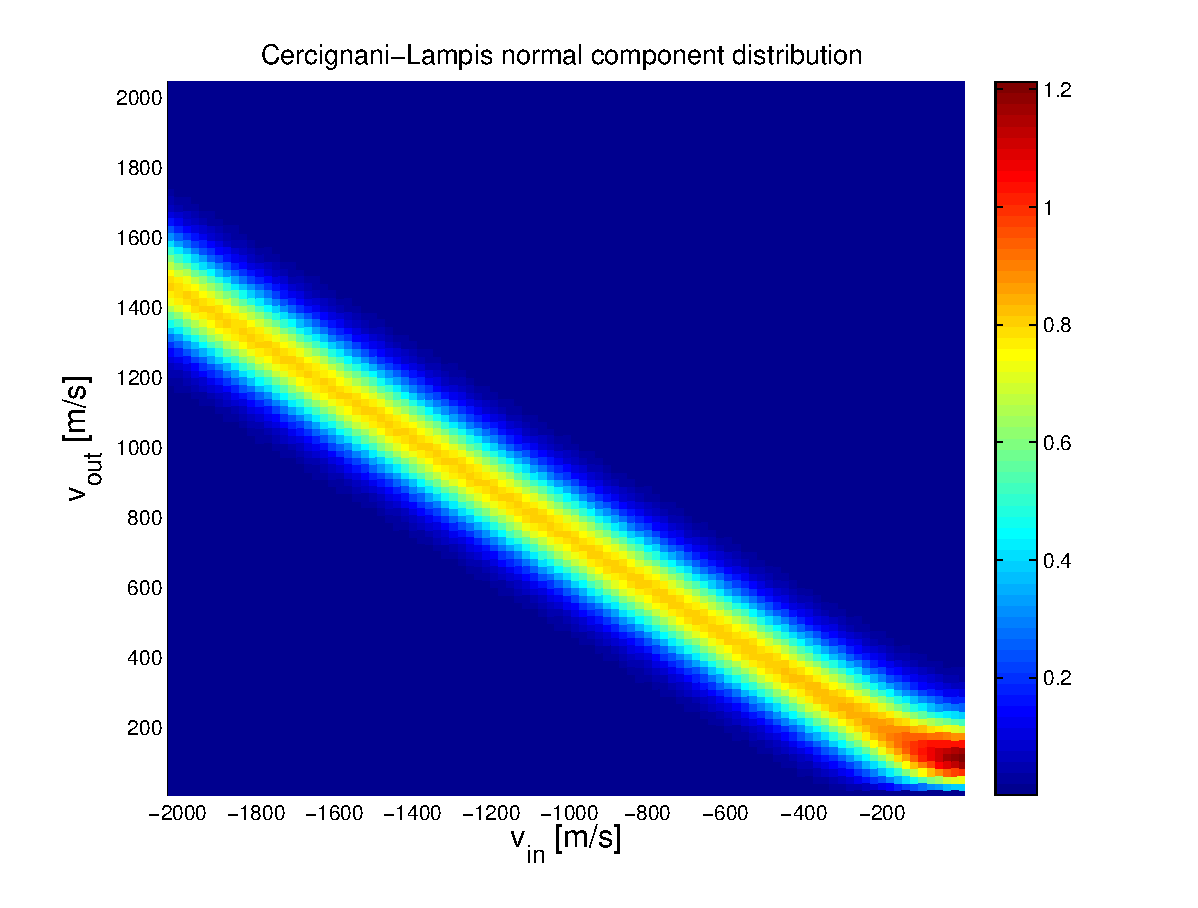
\includegraphics[width=\textwidth, trim=0cm 0cm 0cm 0cm, clip]{DSMC/figures/cercignani-lampis.eps}
\label{fig:cercignani_lampis}
\end{center}
\caption{The Cercignani-Lampis normal component distribution for $T=100K$, $m=m_{argon}$, $\alpha_n=0.5$. We see that particles with high velocities are reflected with a slightly lower velicities converging towards the velocity corresponding to the wall temperature $T_w$.}
\end{figure}

To draw random numbers from this distribution is orders of magnitudes more expensive than the thermal wall since it isn't trivial to invert the cumulative distribution function. Instead we must use the von Neumann algorithm which is a Monte Carlo technique\cite{allen1989computer}. I have implemented and tested this method, but due to the computational cost, the main focus in this thesis is the thermal wall which is used in all the results. 
  \section{Complex geometries}
\label{sec:dsmc_complex_geometries}
All the surface interaction models from section \ref{sec:surface_interactions} use the surface normal and tangent vectors to calculate the reflected velocities. These vectors are easy to determine if the system consists of two parallel plates in the xy-plane, or any other mathematically well described geometry. Such systems are interesting as validation test cases, but most real world materials have a more complex geometry without any simple mathematical description. A very much used representation of such geometries is a triangle mesh in which the surface consists of many connected triangles. The triangles have a well defined normal vector and tangent plane which is easy to calculate. With this method, collision detection is done by checking intersection with each triangle and is rather computationally expensive. In this thesis, I have chosen another approach by representing the system as a large, binary three-dimensional matrix consisting of voxels, each having the value \textit{filled} or \textit{empty}. With this model, collision detection is done by a quick memory lookup to check if the voxel corresponding to the position of a particle is filled or not. In this section we discuss how to create such a matrix, how to identify the surface points and how to calculate the vectors describing the surface geometry.

\subsection{Binary representation - voxels}
\label{sec:dsmc_binary_representation}
With this method, any system geometry is fully described by a three dimensional matrix with dimensions $m\times n\times l$. Each matrix element represents a voxel in the physical space, and can take values 0 or 1. A value of one means that the voxel is filled, whereas zero means empty. No particles can be inside a filled voxel, so this is how we do surface collision detection. 
\subsection{Collision detection}
We define a collision as whether or not a particle has moved into a wall during the timestep $\Delta t$. This has to be checked for every particle each timestep, and in the case of a collision, we need to calculate the resultant velocity. The collision detection algorithm is best illustrated by a code example:
\begin{lstlisting}
bool did_collide(double *position) {
	int voxel_index_i = position[0] / system_length[0] * num_voxels[0];
	int voxel_index_j = position[1] / system_length[1] * num_voxels[1];
	int voxel_index_k = position[2] / system_length[2] * num_voxels[2];

	// The world matrix is a binary matrix
	return world_matrix[voxel_index_i, voxel_index_j, voxel_index_k];
}
\end{lstlisting}
This is just a quick memory lookup. The really expensive part of the full collision algorithm is finding exactly which voxel is the first surface voxel the particle hits. We need to precalculate all the surface voxels so they are marked in the matrix during runtime.
\subsection{Identifying the surface voxels}
Given the binary matrix, we have identified every solid part of the system. The voxels inside a wall that are not part of the surface all have neighbouring voxels that are also marked as walls. We \textit{define} the surface as the filled voxels that have less than 26 neighbouring filled voxels. The algorithm could be implemented like this (one would also have to take care of the periodic boundary conditions, but that is not important to illustrate the idea):
\begin{lstlisting}
bool is_surface(short ***world_matrix, int voxel_index_i, int voxel_index_j, int voxel_index_k) {
	for(int i=-1;i<1;i++) {
    	for(int j=-1;j<1;j++) {
			for(int k=-1;k<1;k++) {
				// Skip self
				if(i == j == k == 0) continue; 
                if(world_matrix[voxel_index_i + i][voxel_index_j + j][voxel_index_k + k] == 0) {
                	// This neighbour is empty
                	return true;
                }
            }
        }
    }

    return false;
}
\end{lstlisting}
This has to be done for every voxel in the system, but only once per system. 
\subsection{Calculating normal and tangent vectors}
The last surface properties we need to calculate are the normal and tangent vectors. This could in principle be done by using marching cubes \cite{article:marching_cubes_original} or a similar technique. However, in this thesis, I have chosen to develop a new way of describing the surface vectors. A cube consisting of 9 voxels has a geometric center $\vec r_{gc}$, plus a center of mass $\vec r_{cm}$ which can be defined through the values, the mass, of the voxels
\begin{align}
	\vec r_{cm} = \sum_i\sum_j \vec r_{ij}m_{ij},
\end{align}
where $m_{ij} \in \{1,0\}$. We \textit{define} the normal vector to be 
\begin{align}
	\vec n = 
\end{align}
\subsection{Scaleability}
  \section{Pressure driven flows}

\subsection{Gravity}
\subsection{Real pressure}

  \section{Parallelization}
% Keywords: MPI, spatial domain geometry, communication surface, 6 facets, world geometry, 
Since there are no long range forces, each collision cell is completely independent. This property makes the model embarrassingly parallel. We divide the spatial domain into subdomains, each fully controlled by one processor. 
\subsection{}
  \section{Code}
  \section{Code validation}
Every time a physicist implement a model, it is important to verify that the implementation is correct. New models that describe unknown areas of physics (such as new length scales) might be difficult to confirm if there are no experiments or comparable models available. 
\subsection{Velocity distribution}
The Poiseuille flow through a long channel is a standard and fundamental problem that is wideley studied in the gas dynamics literature. The system consists of two infinite parallel plates, displaced by a distance $h$. A pressure gradient is applied in the $z$-direction by a constant force $g$, see figure \ref{fig:dsmc_validation_poiseuille}. 

\begin{figure}[htp]
\centering
%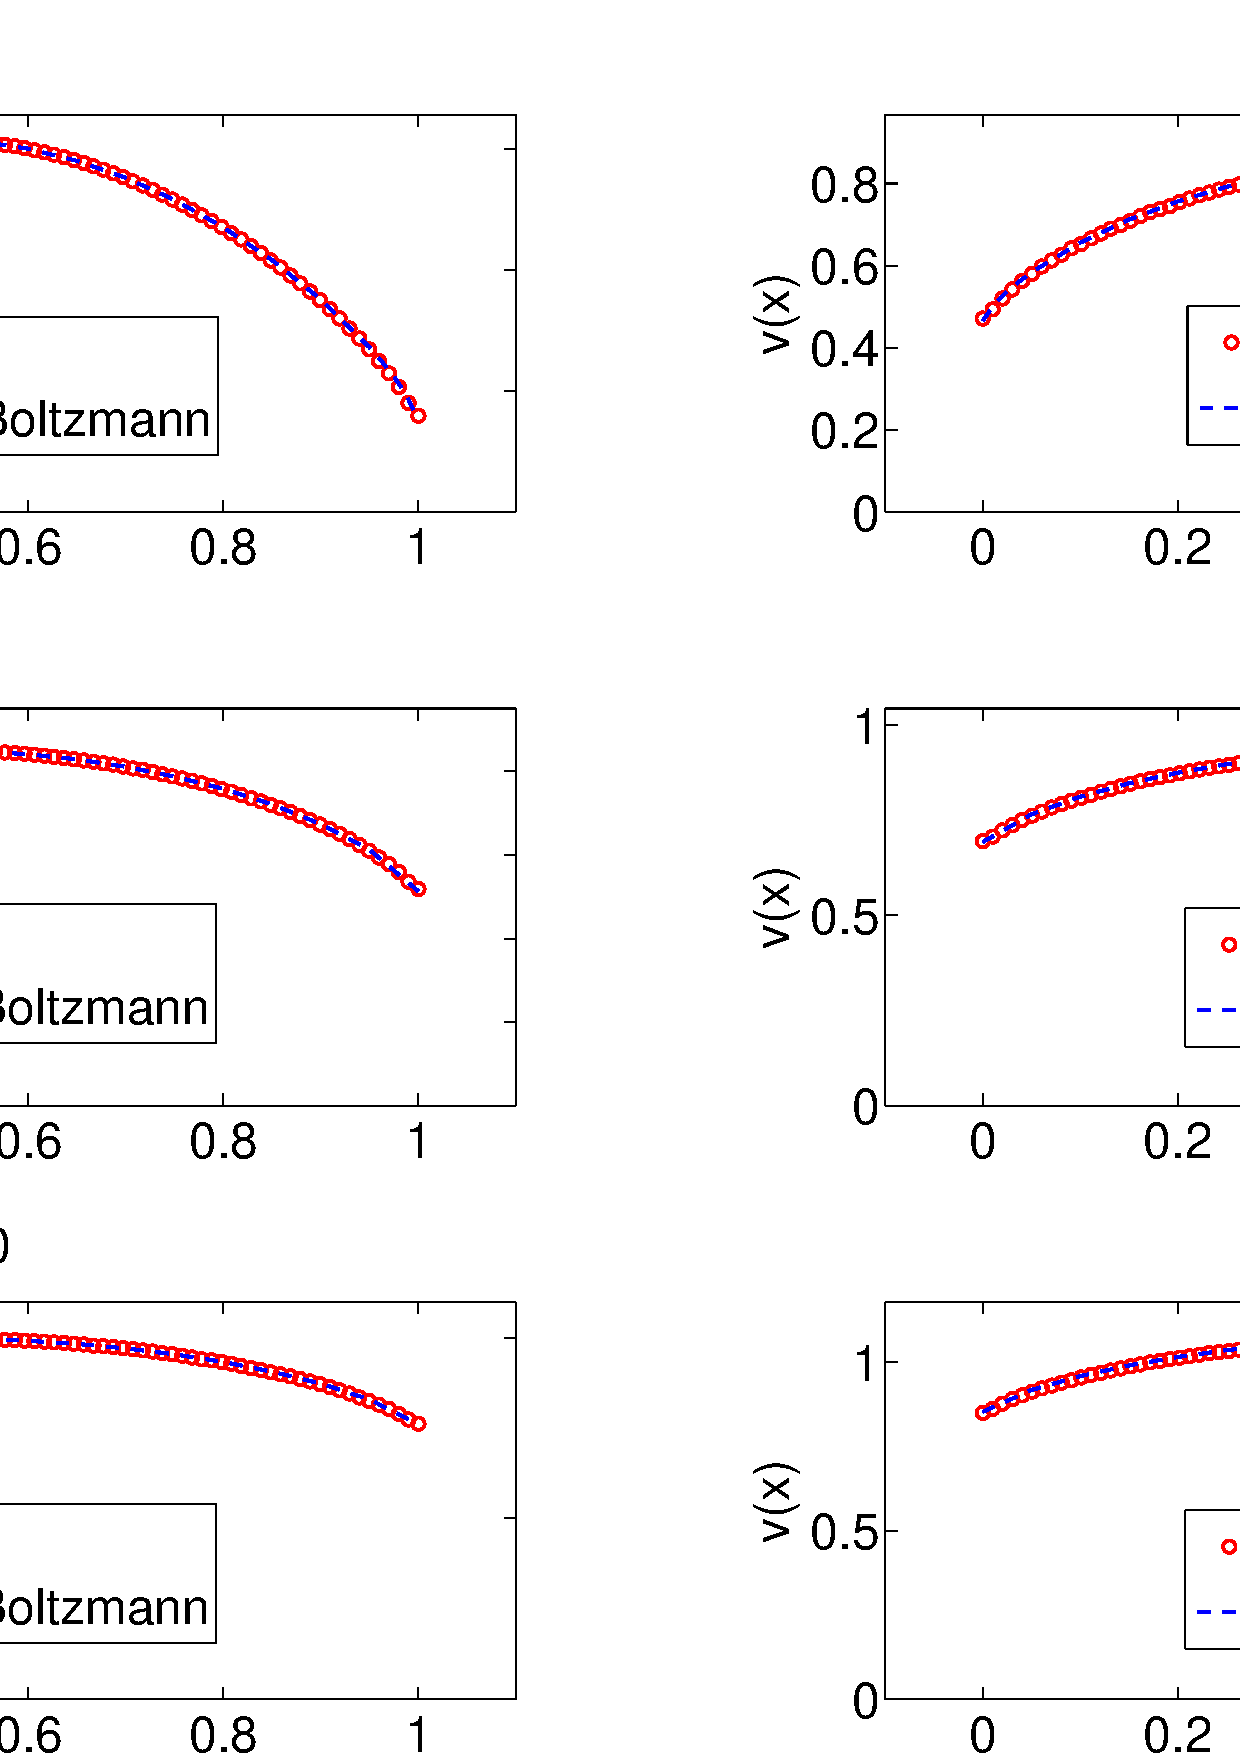
\includegraphics[scale=0.25]{figures/validation_poiseuille.pdf}
\label{fig:dsmc_validation_poiseuille}
\caption{Gravity driven Poiseuille flow}
\end{figure}

The channel is periodic in the $x-$ and $z-$direction, emulating a large system with negligible boundary effects. The gas molecules collide with the plates through the thermal wall model, so the reflected particles will have zero tangential velocity on average. In the continuum limit, $Kn\rightarrow 0$, we expect the velocity profile to approach the parabolic solution \cite{batchelor2000introduction}
\begin{align}
	v_z(y) = \nabla P\frac{1}{2\mu}y(y-h).
\end{align}
However, in the transition flow regime, $0.1 \leq Kn \leq 10$, we expect a non zero slip velocity\cite{morris1992slip}. 

The Knudsen number will affect the velocity distribution through the fact that a high Knudsen number means a larger mean free path, hence fewer inter-molecular collisions. A low collision rate will make the surface effects propagate slower through the system. We therefor expect a larger difference 

\subsubsection{Gravity driven flow}

\end{chapter}
\end{part}

\begin{part}{Visualization}

\end{part}
%---------------------------------------------------------------------------------------
% Appendices
%---------------------------------------------------------------------------------------
\begin{appendices}

\end{appendices}

%---------------------------------------------------------------------------------------
% Bibliography
%---------------------------------------------------------------------------------------
\printbibliography
\end{document}